\newpage

\section{Actividad 4: Característica de salida del JFET}

\subsection{Simulación}

El circuito a implementar es el mismo que antes, con la diferencia de que la fuente de Voltaje V2 ahora variará, obteniendo lo siguiente:

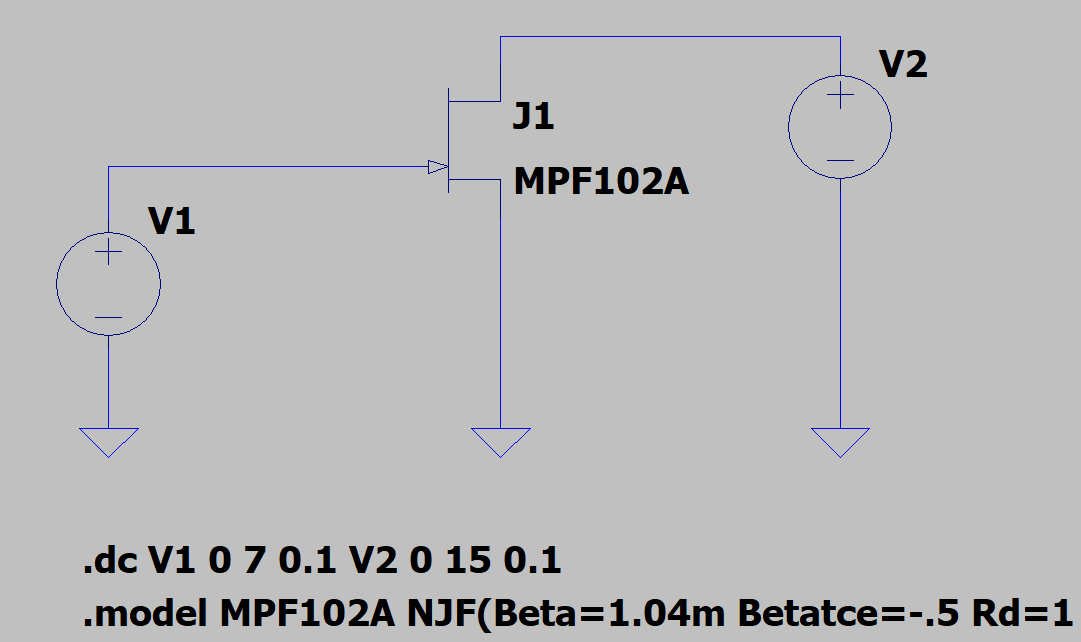
\includegraphics[width=6cm]{./imagenes/Circ4.png}

\subsection{Laboratorio}

\paragraph{Instrumental y Materiales}
\begin{itemize}
    \item Multimetro UNI-T UT89X
    \item Transistor JFET MPF102
    \item Resistor de
    \item Fuente de alimentación
\end{itemize}

\paragraph{Procedimiento}

